\documentclass[a4paper,12pt]{article}
\usepackage{siunitx}
\usepackage[utf8]{inputenc} 
\usepackage{amsmath}
\usepackage{xcolor}
\usepackage{graphicx}
\usepackage[citecolor=blue]{hyperref}       % Para enlaces en el documento
\usepackage{fancyhdr}
\usepackage{circuitikz}
\usepackage{amssymb}
\usepackage{animate}
\usepackage{float}
\usepackage{multirow}
\usepackage{pgfplots}
\usepackage[a4paper, margin=1in]{geometry}
\usepackage{gensymb}
\usepackage{booktabs}
\usepackage{listings}

% Ajuste de la altura del encabezado
\setlength{\headheight}{76.27646pt}
\addtolength{\topmargin}{-34.27646pt}

\lstdefinestyle{mystyle}{
    language=Matlab,
    inputencoding=utf8, % <-- AQUÍ ESTÁ LA CORRECCIÓN
    backgroundcolor=\color{black!5},
    commentstyle=\color{green!60!black},
    keywordstyle=\color{blue},
    numberstyle=\tiny\color{gray},
    stringstyle=\color{purple},
    basicstyle=\footnotesize\ttfamily,
    breaklines=true,
    captionpos=b,
    keepspaces=true,
    numbers=left,
    numbersep=5pt,
    showstringspaces=false,
}
\lstset{style=mystyle}

\setlength{\parindent}{0pt}


% Crear la portada manualmente
\begin{document}

% Desactivar la numeración de página para la portada
\thispagestyle{empty}

% Colocar las imágenes en las esquinas superiores
\begin{minipage}[t]{0.4\textwidth}
    \raggedright
    
\includegraphics[width=2cm]{image/der.png}
\end{minipage}%
\begin{minipage}[t]{0.5\textwidth}
    \raggedleft
    
\includegraphics[width=2cm]{image/izq.png}
\end{minipage}

\vspace{1cm}

\begin{center}
    \Huge{\textbf{Previo 1. Construcción de cables UTP para conexión directa y cruzada.}} \\
    \vspace{2cm}
    \Large{\textbf{Universidad Nacional Autonoma de Mexico.}}\\
    \Large{\textbf{Facultad de ingeniería.}}\\
    \vspace{1cm}
    %\Large{Departamento de Ing. en Control y Robotica.} \\
    %\vspace{0.5cm}
    \Large{Laboratorio de Redes de datos seguras.} \\
    \vspace{0.5cm}
    \LARGE{\textbf{Profesora:}}
    \LARGE{\textit{MTRA. MARIA EUGENIA BAUTISTA GONZALEZ.}}\\
    \vspace{0.5cm}
    \Large{\textbf{Grupo:} 2} \\
    \vspace{0.5cm}
    \LARGE{\textbf{Alumno:}}\\
    \Large{320060829} \\
    %\vspace{0.5cm}
    %\Large{\textbf{Brigada:}}
    %\Large{06} \\
    %\vspace{0.5cm}
    \vspace{3cm}
    \Large{\textbf{Fecha de Entrega:}}\\
    \vspace{0.5cm}
    \large{{Febrero 12, 2026}}
\end{center} 


\newpage

% Configuración del encabezado y pie de página
\pagestyle{fancy}
\fancyhf{}
\fancyhead[L]{
\includegraphics[width=1.5cm]{image/izq.png}}
\fancyhead[R]{
\includegraphics[width=1.5cm]{image/der.png}}
\fancyfoot[C]{\thepage}  % Coloca el número de página en el centro del pie de página

% Línea horizontal en el pie de página
\renewcommand{\footrulewidth}{0.4pt}  % Define el grosor de la línea en el pie de página

% Empezar numeración de páginas desde 1 en la segunda página
\pagenumbering{arabic}
\setcounter{page}{1}

%\maketitle
\tableofcontents

\newpage

\section{Explique la razón por la cual los alambres del cable UTP están trenzados.}

Los alambres del cable UTP estan trenzados para reducir la inteferencia electromagnetica y diafonica, esto es por que cualquier corriente electrica que fluye a traves de un conductor genera un campo magnetico a su alrededor, lo que hace que el cable sea suceptible a inteferencias.

Existen dos tipos:

\begin{enumerate}
    \item Trenzado par a par: cada par de alambres esta trenzado entre si, esto ayuda a cancelar las interferencias electromagneticas, ya que las interferencias afectan ambos alambres de manera similar, lo que permite que las señales se cancelen mutuamente.
    \item Trenzado global: el cable completo esta trenzado, esto ayuda a reducir la diafonia, que es la interferencia entre los pares de alambres dentro del mismo cable.
\end{enumerate}

Los cables UTP operan bajo el principio de la \textbf{señalizacion diferencial}, esto hace que no se envia un voltaje absoluto si no que un cable lleva un voltaje positivo y otro cable lleva un voltaje negativo, esto hace que las interferencias afecten ambos cables de manera similar, lo que permite que las señales se cancelen mutuamente.

\[
\text{Señal}_{\text{Final}} = \left(\text{Señal}_{\text{Positiva}} + \text{Ruido}\right) - \left(\text{Señal}_{\text{Negativa}} + \text{Ruido}\right)
\]

\newpage

\section{¿Qué es un par trenzado: UTP (UnShielded Twisted Pair) cable par trenzado no blindado (no apantallado)?. Explique las características así como ventajas y desventajas.}

Un par trenzado (UTP) es un cable de red que lo que es en si son cables trenzados entre si, pero la diferencia principal es que no tiene una capa de proteccion, esto hace que sea tanto de forma mas barato como fragil, de esto se deberian las ventajas y desventajas de este mismo, donde:

\begin{enumerate}
    \item Caracteristicas:
    \begin{itemize}
        \item Es un cable economico.
        \item Son compatibles con multiples aplicaciones como lo son para redes personales hasta las de area local o LAN.
        \item El diseño de estos cables hace que sean compatibles con distintos tipos de conectores y adaptadores.
        \item Los cabvles UTP son ideales para la instalciones directas de dispositivos sin la nececidad de un concentrador o switch.
    \end{itemize}
    \item Ventajas:
    \begin{itemize}
        \item Es mas barato que los cables blindados, esto hace que el cable sea mas delgado y mas maleable.
        \item La instalacion es mas facil por su flexibilidad, lo que hace que se amas facil de manejar.
        \item Es adecuado para ambientes con baja interferencia electromagnetica, como oficinas o hogares.
    \end{itemize}
    \item Desventajas:
    \begin{itemize}
        \item Al no tener el blindaje, es susceptible a interferencias electricas, lo que puede afectar la calidad de la señal y la velocidad de transmision.
        \item La inmunidad del ruido depende si o si, del equilibrio del trenzado.
        \item No es adecuado para ambientes con alta interferencia electromagnetica, como cerca de motores o equipos de alta potencia.
        \item No es adecuado para largas distancias, ya que la señal se degrada mas rapidamente que en los cables blindados.
    \end{itemize}
\end{enumerate}
\newpage
\section{¿Qué es un par trenzado: STP (Shielded Twisted Pair) cable de par trenzado blindado (apantallado)? Explique las características así como ventajas y desventajas.}

El par tranzado STP es un cable que lo que hace es que tienme barreras conductoras esto lo tiene para aislar los datos del ruido electromagnetico.

\begin{enumerate}
    \item Caracteristicas:
    \begin{itemize}
        \item La capa metalica que actua como blindaje esto lo que hace es actuar como jaula de faraday, esto hace que el cable sea mas resistente a las interferencias electromagneticas.
        \item El blindaje puede ser de diferentes tipos, como el blindaje global, que cubre todo el cable, o el blindaje individual, que cubre cada par de alambres por separado.
        \item El cable STP es ideal para ambientes con alta interferencia electromagnetica, esto es como entornos industriales u hospitales.
    \end{itemize}
    \item Ventajas:
    \begin{itemize}
        \item El blindaje proporciona una mejor proteccion contra las interferencias electromagneticas, lo que mejora la calidad de la señal y la velocidad de transmision.
        \item En la variante S/FTP cada par tiene su propia capa de blindaje, esto hace que sea la proteccion mas alta.
        \item Es adecuado para largas distancias, ya que la señal se degrada menos rapidamente que en los cables UTP.
    \end{itemize}
    \item Desventajas:
    \begin{itemize}
        \item Es mas caro que los cables UTP, esto hace que el cable sea mas grueso y menos maleable.
        \item Para el blindaje funcione correctamtne, debe de estar conectado a tierra fisica de baja impedancia.
        \item La instalacion es mas dificil por su rigidez, lo que hace que sea mas dificil de manejar.
        \item No es adecuado para ambientes con baja interferencia electromagnetica, como oficinas o hogares, ya que el costo y la complejidad de la instalacion no se justifica.
    \end{itemize}
\end{enumerate}

\newpage
\section{Mencione las categorías de cables UTP que existen. Explique más a detalle las principales aplicaciones de los cables de la categoría UTP 5e (5 enhance - mejorada) y UTP 6.}

Las categorias de cables UTP que existen son:
\begin{itemize}
    \item Categoria 1 (solo voz) y 2 (4 Mbps): Son categorias obsoletas, estas se utilizaban para telefonia y redes de baja velocidad.
    \item Categforia 3: Es una de las categorias mas utilizadas para la redes telefonicas, esto es por que soporta las frecuencias de 16 MHz y velocidades de hasta 10 Mbps.
    \item Categoria 4: Por muy poco tiempo fue usado para áreas locales de Token Ring, este cable soporta las velocidades de 16 Mbps y frecuencias de hasta 20 MHz.
    \item Categoria 5: Es una de las categorias mas utilizadas para redes de area local, esto es por que soporta las frecuencias de 100 MHz y velocidades de hasta 100 Mbps.
    \item \textbf{Categoria 5e:} Esta se hizo como una mejora del Cat5 original, esto para permitir la transmision Gigabit completa.
    \begin{itemize}
        \item Ancho de banda: 100 MHz. (frecuencia).
        \item Velocidad de transmision: Hasta 1 Gbps (Gigabit Ethernet) hasta 100 metros.
        \item Aplicaciones: Es ampliamente utilizado en redes de area local (LAN) para conectar computadoras, impresoras, y otros dispositivos de red. Es adecuado para aplicaciones que requieren velocidades de hasta 1 Gbps, como la transmision de video en alta definicion y juegos en linea, asi como telefonia IP, todo esto por que no se prevee flujo masico de datos internos.
        \item Limitaciones: Su construcción (calibre 24 AWG típicamente).
    \end{itemize}
    \item \textbf{Categoria 6:} Esta categoria se hizo como una mejora del Cat5e, esto para permitir la transmision de datos a velocidades de hasta 10 Gbps.
    \begin{itemize}
        \item Ancho de banda: 250 MHz. (frecuencia).
        \item Velocidad de transmision: Hasta 10 Gbps (10 Gigabit Ethernet) hasta 55 metros, y hasta 1 Gbps hasta 100 metros.
        \item Aplicaciones: Es utilizado en redes de area local (LAN) para aplicaciones que requieren velocidades de hasta 10 Gbps, como la transmision de video en alta definicion, juegos en linea, y aplicaciones empresariales que requieren un alto rendimiento.
        \item Limitaciones: Su construcción (calibre 23 AWG típicamente), lo que hace que sea mas rigido y menos maleable que el Cat5e, lo que puede dificultar su instalacion en espacios reducidos o con curvas pronunciadas.
        \item Los cables CAT 6a se utilizan en edificios y proyectos industriales  que tienen una infraestructura de telecomunicaciones a gran escala. Sin embargo, pueden llegar a una distancia máxima del cableado principal de 100 m.
    \end{itemize}

    \item Categoria 6a: Es una mejora del Cat6, esto para permitir la transmision de datos a velocidades de hasta 10 Gbps a distancias de hasta 100 metros. (500 MHz).
    \item Categoria 7: Es una mejora del Cat6a, esto para permitir la transmision de datos a velocidades de hasta 10 Gbps a distancias de hasta 100 metros, ademas de tener un blindaje adicional para reducir las interferencias electromagneticas. (600 MHz).
    \item Categoria 8: Es la categoria mas alta, esto para permitir la transmision de datos a velocidades de hasta 40 Gbps a distancias de hasta 30 metros, ademas de tener un blindaje adicional para reducir las interferencias electromagneticas.(2000 MHz).
\end{itemize}
\section{¿Qué categoría de cable UTP es conveniente utilizar en nuevas instalaciones de cableado y por qué?}

La categoría de cable UTP más conveniente para utilizar en nuevas instalaciones de cableado
estructurado es Cat 6 o, preferentemente, Cat 6a. Estas categorías ofrecen un mayor
desempeño que el Cat 5e, ya que están diseñadas para soportar velocidades más altas y un
mayor ancho de banda, lo cual es fundamental para las redes modernas que manejan grandes
volúmenes de información.

El cable Cat 6 puede trabajar a velocidades de hasta 10 Gbps en distancias cortas
(aproximadamente 55 metros) y a 1 Gbps hasta 100 metros, mientras que el Cat 6a soporta
10 Gbps hasta los 100 metros completos. Esto permite que la red esté preparada para
aplicaciones exigentes como videoconferencias, streaming en alta definición, servidores,
almacenamiento en red y sistemas empresariales.

Además, estas categorías ofrecen una mejor protección contra interferencias y diafonía, lo
que se traduce en una señal más estable y con menos errores. Esto es muy importante en
entornos donde existen muchos equipos eléctricos y electrónicos funcionando al mismo
tiempo.

Aunque el costo del cable Cat 6 o 6a es un poco mayor que el del Cat 5e, esta inversión se
justifica porque el cableado se utiliza por muchos años. Elegir una categoría superior evita
tener que rehacer la instalación en poco tiempo y garantiza que la red pueda crecer y
adaptarse a futuras necesidades tecnológicas.

\newpage
\section{Mencione las características de otros medios de transmisión: el cable coaxial y la fibra óptica.}

\begin{enumerate}
    \item Cable coaxial
    \begin{itemize}
        \item La estructura del cable coaxial es donde un nucleo central de cobre solido, rodeado por un aislante dielectrico grueso, luego una malla de cobre trenzada que actua como blindaje, y finalmente una cubierta exterior de plastico.
        \item El cable coaxial es utilizado para la transmision de señales de television por cable, internet de banda ancha, y redes de area local (LAN) en entornos empresariales.
        \item Este es suceptible a interferencias electromagneticas, pero el blindaje ayuda a reducir estas interferencias, lo que mejora la calidad de la señal.
        \item Los cables coaxiales son líneas de transmisión eléctrica utilizadas para pasar señales de alta radiofrecuencia.
    \end{itemize}
    \item Fibra optica
    \begin{itemize}
        \item Transmite datos mediante pulsos de luz (fotones) a través de fibras de vidrio o plástico, lo que permite velocidades de transmisión muy altas y una mayor capacidad de ancho de banda en comparación con los cables de cobre tradicionales.
        \item La estructura de la fibra optica es donde un nucleo central de vidrio o plastico, rodeado por una capa de revestimiento que tiene un indice de refraccion menor que el nucleo, y finalmente una cubierta exterior de plastico.
        \item La fibra optica es utilizada para la transmision de datos a larga distancia, como en redes de area amplia (WAN), y para la transmision de señales de television por cable.
        \item La fibra optica es inmune a las interferencias electromagneticas, lo que mejora la calidad de la señal y permite velocidades de transmision muy altas.
        \item La fibra optica es un medio de transmision que utiliza pulsos de luz para transmitir datos a traves de fibras de vidrio o plastico, lo que permite velocidades de transmision muy altas y una mayor capacidad de ancho de banda en comparacion con los cables de cobre tradicionales.
        \item Esta misma tambien ofrece un latencia muy baja, lo que la hace ideal para aplicaciones que requieren una respuesta rapida, como los juegos en linea y las videoconferencias.
        
    \end{itemize}
\end{enumerate}
\newpage
\section{Si se va a tender un cable que transmita voz a través de cable UTP ¿Qué pines se utilizarían, cómo se armaría?}
Para la transmisión de voz analógica a través de un cable UTP utilizando conectores RJ45, se emplean los pines centrales del conector, específicamente los pines $4$ y $5$. Según las normas de cableado estructurado T568A y T568B, estos pines corresponden al par de color Azul y Blanco-Azul (donde el pin $4$ es habitualmente el color Azul y el pin $5$ el Blanco-Azul). El proceso de armado consiste en retirar aproximadamente $2.5$ cm de la cubierta exterior del cable UTP, destrenzar los pares únicamente lo necesario para alinearlos, colocar el par azul en la posición central (pines $4$ y $5$) asegurando que los demás cables den soporte mecánico o se corten si no se usarán, insertar los conductores a fondo en el conector RJ45 y finalmente utilizar una herramienta de crimpado para fijar los contactos metálicos sobre los hilos de cobre.


\newpage
\section{Investigue la configuración para un cable cruzado en redes de tipo Gigabit Ethernet}

Para implementar una configuración de cable cruzado funcional en redes Gigabit Ethernet (1000BASE-T), es obligatorio realizar el cruce de los cuatro pares de hilos del cable de par trenzado. En este esquema, mientras un extremo del cable se termina típicamente bajo la norma T568B, el extremo opuesto debe reasignar los pines de manera específica para garantizar la sincronización bidireccional en todas las líneas: el pin 1 se conecta al 3, el pin 2 al 6, el pin 3 al 1 y el pin 6 al 2; simultáneamente, los pares restantes se cruzan conectando el pin 4 con el 7, el pin 5 con el 8, el pin 7 con el 4 y el pin 8 con el 5. Esta permutación completa es crítica para soportar el tráfico de alta velocidad entre dispositivos de la misma jerarquía (como de switch a switch) cuando la detección automática Auto-MDIX no está disponible.

\vspace{0.5cm}
Auto-MDIX: Es una función que permite a los dispositivos de red detectar automáticamente el tipo de cable conectado (directo o cruzado) y ajustar su configuración de transmisión en consecuencia, eliminando la necesidad de preocuparse por el tipo de cable utilizado para conectar dispositivos similares o diferentes.

\begin{tikzpicture}[
    pin/.style={circle, draw=black!60, fill=white, inner sep=0pt, minimum size=6mm, font=\bfseries\small},
    wire/.style={line width=2pt}
]

    % Definición de colores de los pares
    \definecolor{c_orange}{RGB}{255, 140, 0}
    \definecolor{c_green}{RGB}{0, 150, 0}
    \definecolor{c_blue}{RGB}{0, 0, 200}
    \definecolor{c_brown}{RGB}{139, 69, 19}

    % Títulos
    \node[font=\bfseries\large] at (0, 9.5) {Extremo A (T568B)};
    \node[font=\bfseries\large] at (8, 9.5) {Extremo B (Gigabit Cross)};

    % Pines Lado Izquierdo (T568B)
    \foreach \i in {1,...,8} {
        \node[pin] (L\i) at (0, 9-\i) {\i};
    }

    % Pines Lado Derecho (Crossover)
    \foreach \i in {1,...,8} {
        \node[pin] (R\i) at (8, 9-\i) {\i};
    }

    % --- CONEXIONES (Cruce Gigabit Completo) ---
    
    % Par Naranja (1 y 2) cruza a Verde (3 y 6)
    \draw[wire, c_orange, dashed] (L1.east) -- (R3.west); % Blanco/Naranja -> Pin 3
    \draw[wire, c_orange]         (L2.east) -- (R6.west); % Naranja -> Pin 6

    % Par Verde (3 y 6) cruza a Naranja (1 y 2)
    \draw[wire, c_green, dashed]  (L3.east) -- (R1.west); % Blanco/Verde -> Pin 1
    \draw[wire, c_green]          (L6.east) -- (R2.west); % Verde -> Pin 2

    % Par Azul (4 y 5) cruza a Marrón (7 y 8)
    \draw[wire, c_blue]           (L4.east) -- (R7.west); % Azul -> Pin 7
    \draw[wire, c_blue, dashed]   (L5.east) -- (R8.west); % Blanco/Azul -> Pin 8

    % Par Marrón (7 y 8) cruza a Azul (4 y 5)
    \draw[wire, c_brown, dashed]  (L7.east) -- (R4.west); % Blanco/Marrón -> Pin 4
    \draw[wire, c_brown]          (L8.east) -- (R5.west); % Marrón -> Pin 5

    % Etiquetas de los cables en el centro (Opcional para claridad)
    \node[font=\tiny, color=gray] at (4, -0.5) {Líneas discontinuas = Hilo "Blanco/Color"};

\end{tikzpicture}

\newpage
\section{¿Qué significan las normas ANSI/EIA/TIA T568-A y ANSI/EIA/TIA T568-B?}
La Asociación de la Industria de las Telecomunicaciones (TIA) y la Asociación de Industrias de Electrónica (EIA), son asociaciones industriales que desarrollan y publican una serie de estándares sobre el cableado estructurado para voy y datos para las LAN.
\begin{enumerate}
    \item ANSI/EIA/TIA T568-A
    \begin{itemize}
        \item El estandar TIA/EIA define la configuracion de los cables de par trenzado para redes LAN, esta norma especifica los requerimientos minimos para el cableado de establecimientos.
        
        Se hacen recomendaciones:
        \begin{itemize}
            \item Topologia 
            \item Distancia maxima de los cables 
            \begin{enumerate}
                \item Una distancia entre ellos de hasta 3 km, usando repetidores.
                \item Un espacio de oficinas de hasta 1000000 metros cuadrados.
                \item Una población de hasta 50000 usuarios individuales.
                \item La distancia entre un repetidor y una estación de trabajo debe ser no mayor a 100 metros.
            \end{enumerate}
            \item Tipos de conectores y cables a utilizar
            \item Requerimientos de rendimiento para el cableado
        \end{itemize}
        Esta fue diseñada para ser retrocompatible con los codigos de color de telefonia USOC de uno y dos pares, esto hace que sea la norma mas utilizada en las instalaciones de cableado estructurado. (EE.UU)
        \begin{itemize}
            \item Orden: Blanco-Verde, Verde, Blanco-Naranja, Azul, Blanco-Azul, Naranja, Blanco-Marrón, Marrón.
        \end{itemize}
    \end{itemize}
    \item ANSI/EIA/TIA T568-B
    
    La norma ANSI/TIA 568B cuenta con tres subdivisiones las cuaLes son:
    \begin{itemize}
        \item ANSI/TIA/EIA-568-B1: Cableado genérico de Telecomunicaciones en Edificios Comerciales. (Requisitos y recomendaciones en estructura, configuración, interfaces, instalación, parámetros de desempeño y verificación )
        \item TIA/EIA 568-B2: Requerimientos generales para componentes de par tranzado balanceados
        \item TIA/EIA 568-B3: Componentes de cableado, fibra óptica (cable, conectores, hardware de conexión, cordones, jumpers y equipo de prueba)
    \end{itemize}
    Esta norma es una alternativa a la T568A, esta fue diseñada para ser retrocompatible con los codigos de color de telefonia USOC de uno y dos pares, esto hace que sea la norma mas utilizada en las instalaciones de cableado estructurado. (EE.UU)
    \begin{itemize}
        \item Orden: Blanco-Naranja, Naranja, Blanco-Verde, Azul, Blanco-Azul, Verde, Blanco-Marrón, Marrón.
        \item Esta norma es la mas utilizada en las instalaciones de cableado estructurado, esto es por que es compatible con los codigos de color de telefonia USOC de uno y dos pares.
    \end{itemize}
    Mezclar A en un extremo y B en el otro crea un cable cruzado, lo que detendrá la comunicación si los equipos no soportan Auto-MDIX.

\end{enumerate}
\newpage
\section{¿Cuál es la importancia de la capa 1 del modelo OSI?}


El modelo OSI (Open Systems Interconnection) divide las comunicaciones en siete capas, siendo la Capa Física (Capa 1) la base fundamental.

Es la conexión de primer nivel entre los dispositivos y proporciona soporte de hardware y conectividad a toda la red. Para profundizar en este tema, es necesario comprender mejor el modelo completo y la función de la capa física en el modelo OSI.

Además de la transmisión propiamente dicha, el physical layer también regula la estructura de los bits, su valor y sus distintos métodos de transmisión.

La capa física se limita a establecer la conexión física, a transmitir todos los datos como un flujo en forma de bits y a garantizar la correcta desconexión al final de la transmisión.


La importancia de la Capa 1 radica en que es el único punto de contacto tangible con el mundo real. Si la Capa 1 falla (cable roto, conector mal crimpado, atenuación excesiva, interferencia EMI), ninguna capa superior puede corregirlo. 
\begin{itemize}
    \item Representación de bits :La capa física del modelo OSI (Capa 1) se encarga de transmitir bits individuales de un nodo a otro a través de un medio físico. Especifica el procedimiento de codificación de bits, como la cantidad de voltios que deben representar un bit 0 y un bit 1 en el caso de señales eléctricas.
    \item Velocidad de datos: La velocidad de datos se mantiene mediante la función de la capa física en el modelo OSI. La cantidad de bits enviados por segundo se denomina velocidad de datos. 
    \item Sincronización: La función de la capa física en el modelo OSI incluye la sincronización de bits. El emisor y el receptor están sincronizados a nivel de bits.
    \item Interfaz: La interfaz de transmisión entre los dispositivos y el medio de transmisión se define por la capa física en el modelo OSI. PPP, ATM y Ethernet son las tres tramas más utilizadas en la interfaz física. 
    \item Configuración de línea: La función de la capa física en los modelos OSI incluye la conexión de dispositivos al medio o configuración de línea. La configuración de línea, también conocida como conexión, es el método mediante el cual dos o más dispositivos se conectan a un enlace. Un enlace dedicado conecta dos dispositivos en una configuración punto a punto.
    \item Topologías: La capa física del modelo OSI especifica cómo deben conectarse entre sí los diferentes dispositivos informáticos de una red. Una topología de red es la configuración mediante la cual se conectan entre sí los sistemas informáticos o dispositivos de red. 
    \item Modos de transmisión: La capa física del modelo OSI especifica la dirección de transmisión entre dos dispositivos. El modo de transmisión se refiere al método utilizado para transferir datos de un dispositivo a otro.
\end{itemize}

\newpage
\section{ Investigue costos del cable UTP categorías 5e, 6 y 6a.}

\subsection*{Categoría 5e (Cat 5e)}
Esta categoría sigue siendo el estándar básico para redes domésticas y pequeñas oficinas en México debido a su bajo costo. Es suficiente para velocidades de hasta 1 Gbps en distancias cortas.

\begin{itemize}
    \item \textbf{Precios encontrados:} En tiendas especializadas como Alcione, el precio de lista por metro ronda los \$20.00 MXN, con ofertas que bajan a \$14.67 MXN \cite{alcione2026}. Por otro lado, distribuidores como Steren manejan un precio al público de \$14.00 MXN por metro, reduciéndose a \$12.75 MXN en compras de mayoreo \cite{steren2026}. En plataformas como Mercado Libre, las bobinas de aleación (CCA) reducen drásticamente el costo técnico a cerca de \$3.00 - \$5.00 MXN el metro, aunque no se recomienda para certificaciones profesionales.
    \item \textbf{Promedio de mercado:} \$17.00 MXN por metro (Corte al menudeo).
\end{itemize}

\subsection*{Categoría 6 (Cat 6)}
La categoría 6 es actualmente el estándar recomendado para nuevas instalaciones empresariales en México, ofreciendo un mejor rendimiento contra la diafonía y soportando 10 Gbps en distancias cortas (hasta 55 metros).

\begin{itemize}
    \item \textbf{Precios encontrados:} En proveedores industriales como Acomee, el cable UTP Cat 6 de marcas reconocidas (como Condumex) oscila entre \$17.28 MXN y \$23.00 MXN por metro antes de impuestos \cite{acomee2026}. Alcione reporta precios de lista de hasta \$27.23 MXN, aunque se pueden encontrar en oferta alrededor de \$13.94 MXN por metro \cite{alcione2026}.
    \item \textbf{Promedio de mercado:} \$21.00 MXN por metro (Corte al menudeo).
\end{itemize}

\subsection*{Categoría 6a (Cat 6a)}
Utilizado para centros de datos, hospitales y aplicaciones que requieren 10 Gbps a 100 metros completos. Su costo es significativamente más alto debido al blindaje adicional y la mayor cantidad de cobre y aislamiento requeridos.

\begin{itemize}
    \item \textbf{Precios encontrados:} Este cable es menos común para venta "por metro" en ferreterías estándar. En Steren, el precio por metro alcanza los \$39.00 MXN \cite{steren2026}. Al adquirirlo por bobina en sitios especializados en infraestructura como Sily o Syscom (marcas Belden o LinkedPro), el costo por bobina de 305m varía entre \$4,300 y \$10,000 MXN, lo que sitúa el costo técnico por metro entre \$14.00 y \$33.00 MXN dependiendo de la calidad del blindaje (UTP vs F/UTP) \cite{sily2026}.
    \item \textbf{Promedio de mercado:} \$39.00 MXN por metro (Corte al menudeo).
\end{itemize}

\section*{Resumen de Promedios}
Basado en la investigación realizada en febrero de 2026 en el área metropolitana y distribuidores en línea de México:

\begin{itemize}
    \item \textbf{Promedio Cat 5e:} \$17.00 MXN / metro.
    \item \textbf{Promedio Cat 6:} \$21.00 MXN / metro.
    \item \textbf{Promedio Cat 6a:} \$39.00 MXN / metro.
\end{itemize}

\begin{thebibliography}{9}
    % Principios Electromagnéticos y Trenzado
    \bibitem{belden_trenzado}
    Belden. (s.f.). \textit{Porque los cables de red UTP están trenzados}. Tecnosinergia. Recuperado de \url{https://tecnosinergia.zendesk.com/hc/es/articles/44727545171355-Porque-los-cables-de-red-UTP-est%C3%A1n-trenzados-BELDEN}

    % UTP vs STP y 10GBASE-T
    \bibitem{fibermart_utp_stp}
    Fiber-Mart. (s.f.). \textit{UTP vs STP Cable in 10GBASE-T Ethernet Cabling}. Recuperado de \url{https://www.fiber-mart.com/es/news/utp-vs-stp-cable-in-10gbaset-ethernet-cabling-a-6593.html}

    % Categorías de Cableado 5e, 6 y 6A
    \bibitem{satpcs_utp}
    SAT PCS. (2025, 23 de diciembre). \textit{Qué es un cable UTP y por qué es tan importante saberlo}. Recuperado de \url{https://satpcs.com/sp/blog/que-es-un-cable-utp-y-por-que-es-tan-importante-saberlo}

    \bibitem{transworld_cat6}
    Transworld. (2025, 3 de noviembre). \textit{Diferencias entre cables Cat 5e, Cat 6 y Cat 6A}. Recuperado de \url{https://www.transworld.cl/i-news/cat5e-vs-cat6-vs-cat6a/}

    % Recomendaciones Nuevas Instalaciones (TIA-568)
    \bibitem{dolph_tia}
    Dolph Microwave. (2026, 23 de enero). \textit{Qué tipos de cable se incluyen en los estándares de cableado estructurado TIA 568}. Recuperado de \url{https://www.dolphmicrowave.com/es/que-tipos-de-cable-se-incluyen-en-los-estandares-de-cableado-estructurado-tia-568/}

    \bibitem{siemon_tia_e}
    Siemon. (2025, 19 de marzo). \textit{ANSI/TIA-568.2-E ya está aquí. ¿Sus cables cumplen la norma?}. Recuperado de \url{https://www.siemon.com/es/ansi-tia-568-2-e-ya-esta-aqui-sus-cables-cumplen-la-norma/}

    % Fibra Óptica vs Coaxial
    \bibitem{rackonline_fibra}
    RackOnline. (2025, 30 de enero). \textit{Fibra óptica vs. cable coaxial: cuál es la mejor opción}. Recuperado de \url{https://www.rackonline.es/blog/fibra-optica/fibra-optica-vs-cable-coaxial-cual-es-la-mejor-opcion}

    \bibitem{wikipedia_medios}
    Wikipedia. (s.f.). \textit{Medio de transmisión}. Recuperado de \url{https://es.wikipedia.org/wiki/Medio_de_transmisi%C3%B3n}

    % Voz y RJ11/RJ45
    \bibitem{fibermart_rj11}
    Fiber-Mart. (s.f.). \textit{RJ11 \& RJ45 Modular Connector Tutorial}. Recuperado de \url{https://www.fiber-mart.com/es/news/rj11-rj45-modular-connector-tutorial-a-996.html}

    \bibitem{showmecables_wiring}
    Johnston, A. (2023, 26 de junio). \textit{RJ11 to RJ45 Wiring Diagram}. ShowMeCables. Recuperado de \url{https://www.showmecables.com/blog/post/RJ11-to-RJ45-Wiring-Diagram}

    % Configuración Cable Cruzado Gigabit
    \bibitem{practical_networking}
    Practical Networking. (s.f.). \textit{Ethernet Wiring}. Recuperado de \url{https://www.practicalnetworking.net/stand-alone/ethernet-wiring/}

    \bibitem{pinoutsguide_crossover}
    PinoutsGuide. (2013). \textit{Ethernet 1Gb crossover cable pinout diagram}. Recuperado de \url{https://www.scribd.com/document/471366098/Ethernet-1Gb-crossover-cable-pinout-diagram-pinoutsguide}

    % Normas T568A vs T568B
    \bibitem{seetronic_rj45}
    Seetronic. (2025, 15 de agosto). \textit{RJ45 Wiring Diagram}. Recuperado de \url{https://seetronic.com/es/blog/rj45-wiring-diagram/}

    % Capa Física OSI
    \bibitem{ionos_osi}
    IONOS. (2023, 3 de febrero). \textit{Capa física: funciones de la primera capa}. Recuperado de \url{https://www.ionos.com/es-us/digitalguide/servidores/know-how/capa-fisica/}

    % Costos de Mercado
    \bibitem{alcione_precios}
    Alcione. (2026). \textit{Cable UTP Blindado FTP Cat6 Azul Bobina 305 M}. Recuperado de \url{https://alcione.mx/cable-utp-blindado-ftp-cat6-azul-bobina-305-m-com6%20a%20ftp%20lv}

    \bibitem{mercadolibre_utp}
    Mercado Libre. (2025). \textit{Listado de Cable UTP Cat 6}. Recuperado de \url{https://listado.mercadolibre.com.mx/utp-cat-6}

    \bibitem{alcione2026}
    Alcione. (2026). \textit{Cable UTP Cat 5e y Cat 6: Precios y existencias por metro}. Recuperado el 8 de febrero de 2026, de \url{https://alcione.mx}

    \bibitem{acomee2026}
    Acomee. (2026). \textit{Catálogo de productos de conectividad: Cable UTP Condumex por metro}. Recuperado el 8 de febrero de 2026, de \url{https://www.acomee.com.mx}

    \bibitem{steren2026}
    Steren. (2026). \textit{Cables de red a granel: Categorías 5e, 6 y 6a}. Steren Tienda en Línea. Recuperado el 8 de febrero de 2026, de \url{https://www.steren.com.mx}

    \bibitem{sily2026}
    Sily. (2026). \textit{Colección de Cables Categoría 6A y Bobinas Belden}. Recuperado el 8 de febrero de 2026, de \url{https://sily.mx}

\end{thebibliography}

\end{document}